%Tablas hechas con la herramienta http://www.tablesgenerator.com/# cambiando l para p{8cm} para hacer el salto de linea
\documentclass{article}

\usepackage{titlesec}
\usepackage[utf8]{inputenc}
\usepackage{graphicx}
\usepackage{ amssymb }
%\usepackage{subfig}
\usepackage{subcaption}
%\usepackage{breqn}
\usepackage{mathtools,bm}
\usepackage{eurosym}
\usepackage{amstext} % for \text
\DeclareRobustCommand{\officialeuro}{%
  \ifmmode\expandafter\text\fi
  {\fontencoding{U}\fontfamily{eurosym}\selectfont e}}
\usepackage[spanish]{babel} %changes the LaTex default labels to spanish
\usepackage{float} %enables the anchorage of the figures and tables within the text, with [H]
\usepackage{longtable}

\usepackage[a4paper,bindingoffset=0.2in,%
            left=1in,right=1in,top=1in,bottom=1in,%
            footskip=.25in]{geometry}
% \graphicspath{ {images/}, {images2/} }
\usepackage{amsmath}
\usepackage[hyphens]{url}
\usepackage{hyperref}
\usepackage{multirow}


%\setcounter{secnumdepth}{4}

\titleformat{\paragraph}
{\normalfont\normalsize\bfseries}{\theparagraph}{1em}{}
\titlespacing*{\paragraph}
{0pt}{3.25ex plus 1ex minus .2ex}{1.5ex plus .2ex}

\newcommand*{\frontPageEC}[2]{
    \begingroup % Create the command for including the title page in the document
        \centering % Center all text
        \vspace*{\baselineskip} % White space at the top of the page
        {\begin{flushright} \LARGE #1  \end{flushright}}
        \vspace*{\baselineskip}
        \rule{\textwidth}{1.6pt}\vspace*{-\baselineskip}\vspace*{2pt} % Thick horizontal line
        \rule{\textwidth}{0.4pt}\\[\baselineskip] % Thin horizontal line
        {\LARGE #2  \\[0.8\baselineskip] \large{Robótica y Percepción Computacional}}\\[0.2\baselineskip] % Title
        \rule{\textwidth}{0.4pt}\vspace*{-\baselineskip}\vspace{3.2pt} % Thin horizontal line
        \rule{\textwidth}{1.6pt}\\[\baselineskip] % Thick horizontal line
        \vspace*{2\baselineskip} % Whitespace between location/year and editors
        Alumnos: \\[\baselineskip]
        {\Large Luciano García Giordano (150245)} \\
        {\Large Gonzalo Flórez Arias (150048)} \\
        {\Large Salvador González Gerpe (150044)} \\
        
        \vfill
        %\includegraphics[scale=0.4]{UPM.png}
        
        {\itshape Universidad Politécnica de Madrid \\ ETSI Informáticos\par} % Editor affiliation
    \endgroup}

\title{Segmentacion entrega}
\author{Luciano García Giordano, Gonzalo Flórez Arias, Salvador González Gerpe}
\date{24/03/2019}
\date{Universidad Politécnica de Madrid}
\begin{document}

\frontPageEC{24 de marzo de 2019}{Segmentación}
\thispagestyle{empty}

\newpage
\tableofcontents
\setcounter{page}{1}

\clearpage
\newpage

\section{Método. Solución propuesta. Algoritmo de segmentación. Descripción del código desarrollado}

	A la hora de implementar la parte de segmentación, hemos llegado a tomar una serie de decisiones concretas con el objetivo de lograr los mejores resultados posibles. En este sentido, parecen claras las dos vías por las que se puede optimizar un algoritmo de segmentación: mejorar la calidad de la segmentación y mejorar los tiempos de ejecución.

	Nosotros tuvimos, ya desde el primer momento, claro que lo importante sería lograr una buena calidad en la segmentación, y que a partir de ahí el objetivo sería mejorar los tiempos que tarda el algoritmo en proporcionar la segmentación de cierta imagen (ya que en el robot real esto resulta ser importante). 

	Nuestra primera medida, frente al “diseño” original del algoritmo, fue cambiar el espacio de colores de RGB a HSV. A esto unimos el que finalmente nos quedamos solo con H y S, dejando fuera la V (para tratar de evitar problemas con los cambios de iluminación). Esto resultó ser definitivamente importante para lograr un buen clasificador.

	Para etiquetar las imágenes se usó el programa proporcionado por el profesor, que permite colorear un vídeo abierto con OpenCV, por lo que tomamos algunas imágenes y las coloreamos, tratando de obtener datos variados para la línea, el suelo y las marcas. Con esto construimos nuestro dataset de entrenamiento, con unos 30000 píxeles (lo consideramos una cantidad muy elevada, pero hemos obtenido buenos resultados con ello). Almacenamos, de todas las imágenes coloreadas, los canales H y S de los píxeles coloreados para de ahí entrenar el clasificador.

	Respecto al clasificador, aunque la idea inicial era usar un clasificador euclídeo, de manera similar al desarrollado en la asignatura de Reconocimiento de Formas, pensamos que sería ventajoso buscar algo un poco más complejo pero que pudiera separar mejor las clases. Probamos, usando bibliotecas como sklearn, distintas opciones: primero un clasificador gaussiano de tipo Naïve Bayes, luego una red neuronal de 3 capas, luego una de dos capas (haciendo diversas pruebas con distintos números de nodos en cada capa). Nos quedamos finalmente con una red neuronal de 2 capas con 3 nodos en cada una de ellas. Utilizamos activación logística y una tasa de aprendizaje $\alpha$ de 0.05. Con ello obtenemos unos resultados con altos porcentajes de acierto (99.5\% de acierto usando un 90\% de datos de training y un 10\% de datos de test), pero asegurando a la vez una velocidad de ejecución rápida, que se comentará más adelante.

	Así, al ejecutar el programa se ejecuta el entrenamiento pertinente, y posteriormente se va leyendo el vídeo que se deseé segmentar y calculando dicha segmentación, coloreando y mostrando el resultado a la vez. Es posible también hacer esa lectura directamente a partir de una cámara conectada al ordenador.

	Pasan a comentarse ahora las mejoras llevadas a cabo desde la primera entrega de segmentación:

	\begin{itemize}
		\item Gracias a un uso más adecuado de la biblioteca de sklearn, se logró que la ejecución del algoritmo de segmentación fuera paralelizable. De esa manera, no perdemos demasiada potencia de cálculo por utilizar un algoritmo más complejo, como son las redes de neuronas artificiales.
		\item Se pasó a obtener los frames del vídeo de forma reducida. De esa manera, utilizamos para segmentación los píxeles de la imagen de 4 en 4, reduciendo el coste computacional al 1/16 del original. Según nuestras observaciones, casi no se pierde calidad en la segmentación pero se aumenta mucho la velocidad de cómputo.
		\item Se redujeron los nodos en cada capa de la red neuronal, logrando así una velocidad de cómputo mayor sin perder mucha calidad en la segmentación.
		\item Se implementó la parte opcional del seguimiento de la pelota (explicado a continuación).
		\item Como medida para aumentar aún más el acierto en la segmentación, se decidió aumentar la saturación de la cámara a la hora de tomar los vídeos. Según nuestras observaciones, eso hace que los algoritmos funcionen notablemente mejor.
		\item A lo largo de 2 días, tabajamos en el laboratorio de robótica. Allí pudimos grabar y segmentar vídeos tomados desde la propia cámara del robot, con el objetivo de tener ya un vídeo del entorno real de la práctica, además de empezar a probar situaciones reales de seguimiento de líneas en el suelo y de seguimiento de una pelota de ténis.
	\end{itemize}

	Respecto a la implementación de nuestro programa en Python, al comenzar a ejecutar el programa, se llama al clasificador, y se le pide que entrene a partir de los datos del dataset, que se guardan en un fichero (con datasetGenerator se genera este fichero, a partir de las imágenes coloreadas con etiquetaImagenes. Esa generación solo se hace una vez). 

	Se inicia la captura de imágenes, en base a un vídeo concreto (aunque puede realizarse sobre un vídeo en directo desde una cámara). Cada imagen recibida se reduce en un factor de 4, vertical y horizontalmente (no hemos considerado el trabajar con imágenes algo pequeñas un problema para el futuro, pues el tamaño sigue siendo considerable para poder ver correctamente la línea y cada marca), y en un bucle, se van leyendo las imágenes. Se pasa cada imagen al formato HSV, y se obtiene el H y el S. Se clasifica con predict cada pixel de la imagen con el clasificador, y se muestra por pantalla la imagen segmentada. Entre medias se realizan pruebas del tiempo tardado, usadas para el apartado correspondiente de esta memoria.


\section{Resultado. Algoritmo de segmentación}
	% imagenes representativas y tiempos de ejecucion aqui
	Tras probar el algoritmo que tenemos en el robot de la sala de robótica, podemos certificarnos de que funciona bien en un entorno real controlado. Además, podemos asegurarnos de que los tiempos de ejecución son, como mínimo, adecuados. En nuestro caso, la fase de segmentación se hace de tal forma que conseguimos concluirla en 0.01 segundos, lo que nos permite ejecutar muchos frames en cada segundo (serían 77 si el step que implementamos fuera el total del programa). Si ejecutamos el programa que se entrega en este momento, que no es el brain que desarrollamos para probar en el laboratorio de robótica, el tiempo de ejecución de un ciclo es, de media, de 0,013 segundos en un ordenador portátil similar al del robot del laboratorio de robótica (ambos tienen un procesador Intel i3, por ejemplo). La velocidad de la segmentación fue de 77 frames por segundo.

	En cuanto a resultados, mostramos a continuación algunas capturas que hicimos en el laboratorio de robótica controlando manualmente el robot y capturando el vídeo, y luego procesándolo en nuestro programa. En la figura \ref{fig:figura1} se puede ver que la segmentación es correcta. Sin embargo, los bordes de la línea tienen partes rojas. Eso se debe a que no entrenamos el algoritmo con un dataset demasiado separable. Para solucionar este problema, podemos hacer uso de la función erode de openCV, que nos permite eliminar pequeñas regiones mal clasificadas. Otra solución sería hacer un dataset más variado, aunque dado que no consideramos el contexto del píxel como feature en nuestro algoritmo eso puede no ser suficiente. En un brain que hicimos para probar en la sala de robótica para que el robot pudiera seguir líneas, utilizamos la función erode y obtuvimos resultados excelentes.

	\begin{figure}[H]
	    \centering
	    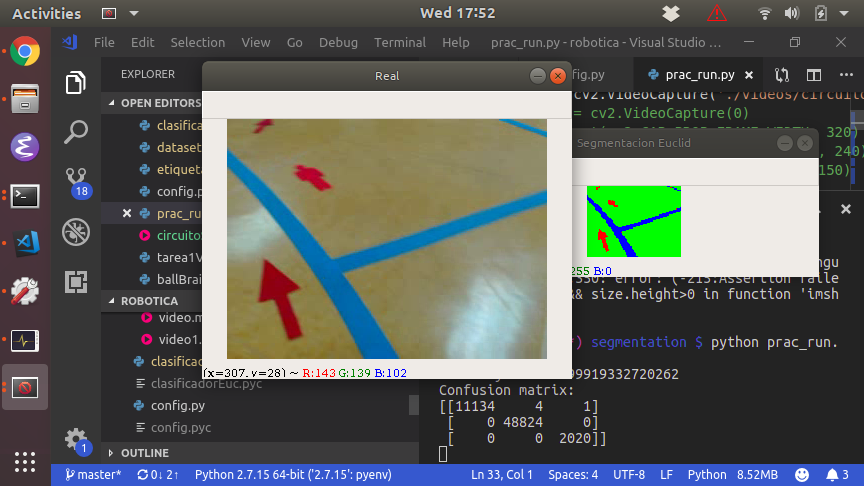
\includegraphics[width=12cm]{figura1.png}
	    \caption{Ejemplo de la segmentación.}
	    \label{fig:figura1}
	\end{figure}

	\begin{figure}[H]
	    \centering
	    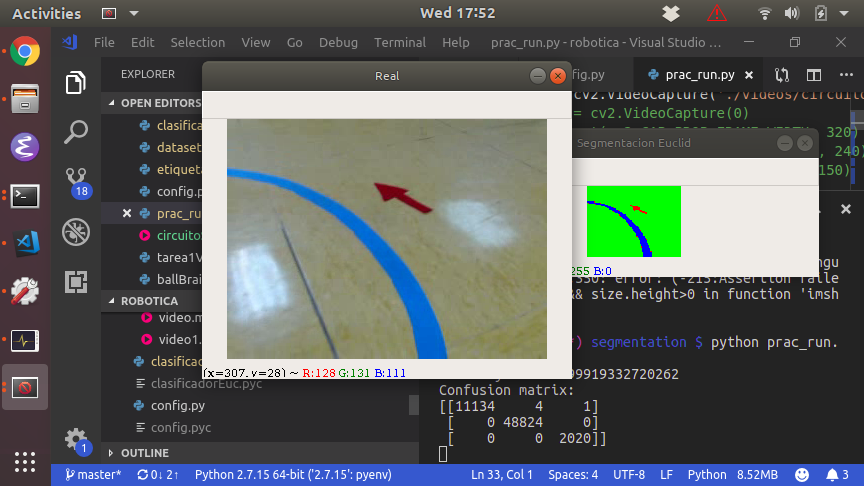
\includegraphics[width=12cm]{figura2.png}
	    \caption{Ejemplo de la segmentación.}
	    \label{fig:figura2}
	\end{figure}

	\begin{figure}[H]
	    \centering
	    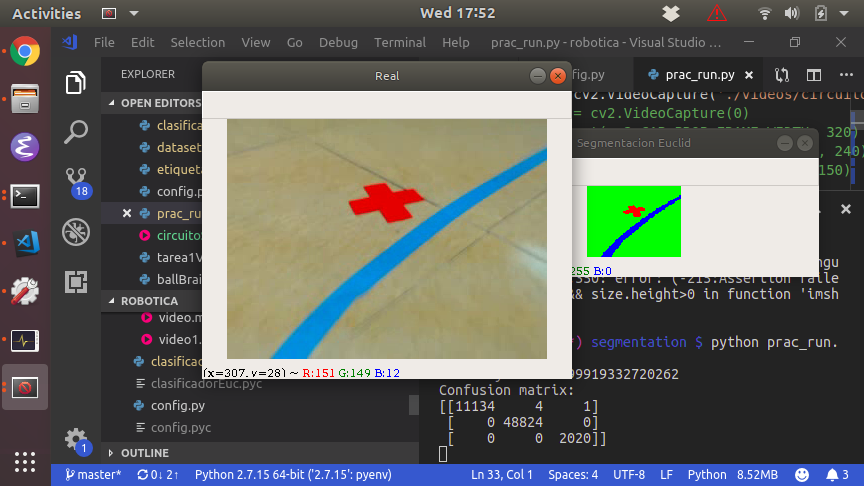
\includegraphics[width=12cm]{figura3.png}
	    \caption{Ejemplo de la segmentación.}
	    \label{fig:figura3}
	\end{figure}

	\begin{figure}[H]
	    \centering
	    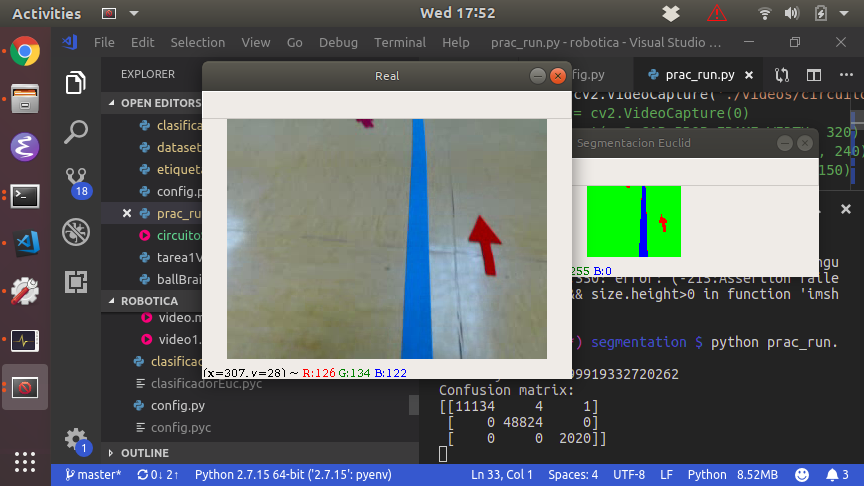
\includegraphics[width=12cm]{figura4.png}
	    \caption{Ejemplo de la segmentación.}
	    \label{fig:figura4}
	\end{figure}



\section{Parte opcional. Seguimiento de pelota}
	También realizamos la parte opcional de la práctica, referida al seguimiento de un objeto esférico por parte del robot, que va controlando su distancia a dicho objeto según los resultados del tamaño de la pelota relativo a la cámara del robot. Logramos adaptar el algoritmo de segmentación para poder obtener la pelota de un vídeo, y calculamos la manera de obtener la distancia relativa de la cámara a la pelota, en base a la explicación dada en clase. También hemos realizado una primera integración de esto con la parte de control, de tal manera que el robot se acerque a la pelota si la encuentra a lo lejos y se aleje si la tiene muy cerca. También implementamos la capacidad del robot de girar para intentar mantener la pelota en el centro de su campo de visión. Probamos el algoritmo en forma de “Brain” en el robot del laboratorio de robótica, logrando unos resultados interesantes. Incluimos en la carpeta de entrega un video de demostración del seguimiento junto con la segmentación hecha por el mismo programa.

	Sobre nuestras pruebas en el laboratorio, incluimos en la carpeta de entrega un timelapse grabado con un móvil de uno de los integrantes del grupo guiando el robot por la sala. Además, incluimos dos videos, uno con la imagen original y otro de la segmentación, hechos en directo por el robot en una situación similar a la mostrada en el time lapse (hemos perdido la referencia de si se trata de la misma ejecución o no). Se muestra a seguir una captura de pantalla del video mencionado, tanto de la imagen original (Figura \ref{fig:pelota1}) como de la segmentación (Figura \ref{fig:pelota2}).

	\begin{figure}[H]
	    \centering
	    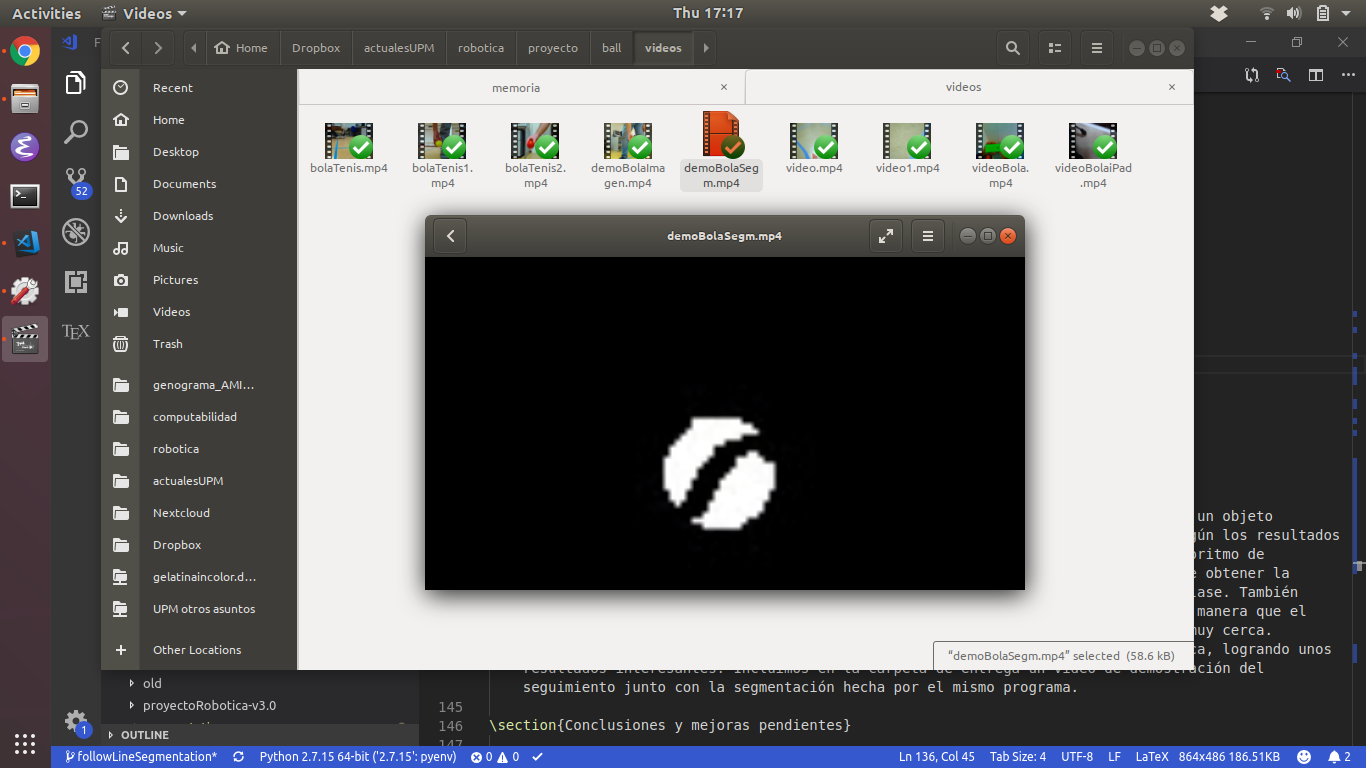
\includegraphics[width=12cm]{pelota1.png}
	    \caption{Captura de la imagen original de la pelota en un brain que ejecuta en el robot real.}
	    \label{fig:pelota1}
	\end{figure}

	\begin{figure}[H]
	    \centering
	    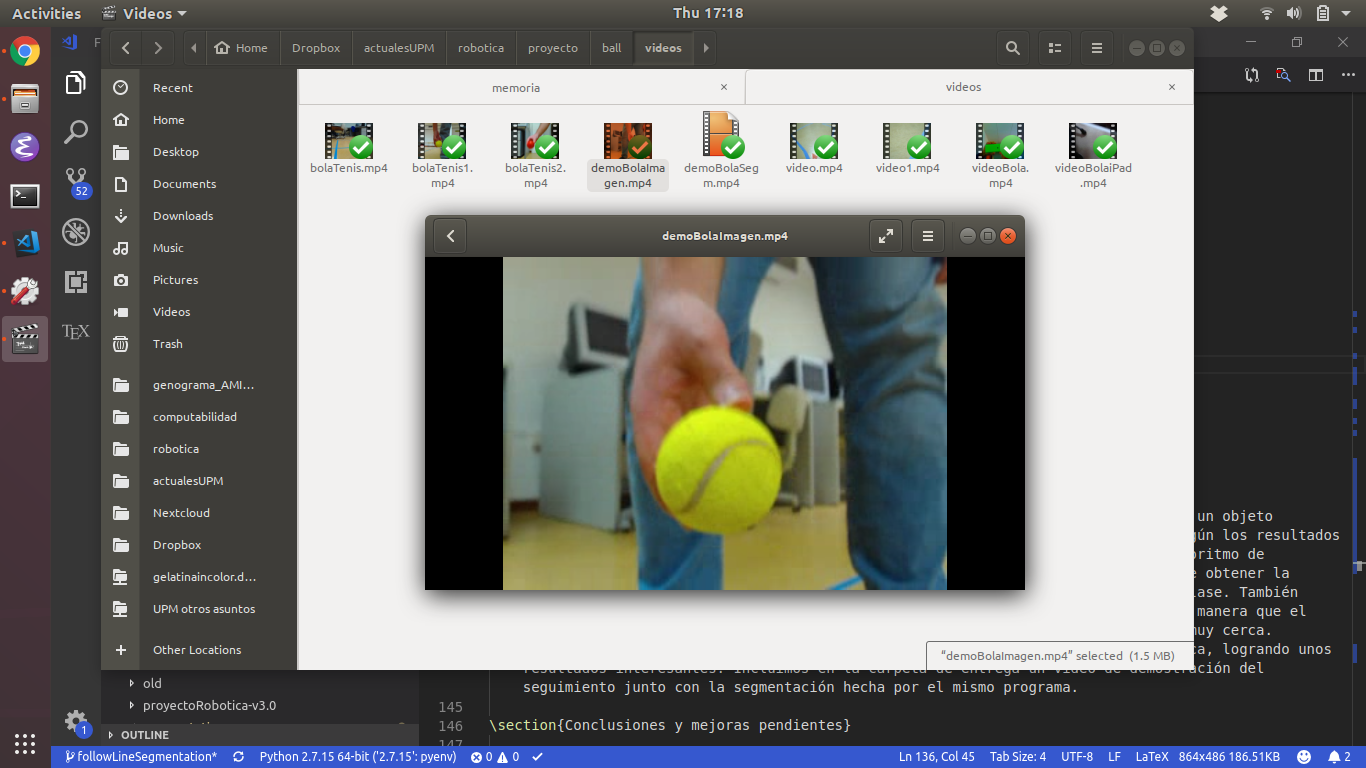
\includegraphics[width=12cm]{pelota2.png}
	    \caption{Captura de la segmentación de la pelota en un brain que ejecuta en el robot real. Como bien se puede ver, hacemos uso de la función erode de openCV para que no se consideren pequeños defectos de la segmentación.}
	    \label{fig:pelota2}
	\end{figure}

\section{Conclusiones y mejoras pendientes}

	Pensamos, en conclusión, que nuestro algoritmo de segmentación obtiene buenos resultados con las pruebas llevadas a cabo. Es cierto que podría ser más rápido (especialmente en nuestra primera versión, de la primera entrega de esta parte), pero hemos tratado de encontrar un equilibrio entre resultados y tiempos de ejecución que nos permita emplear este algoritmo una vez usemos el robot real.









% \begin{figure}[H]
%     \centering
%     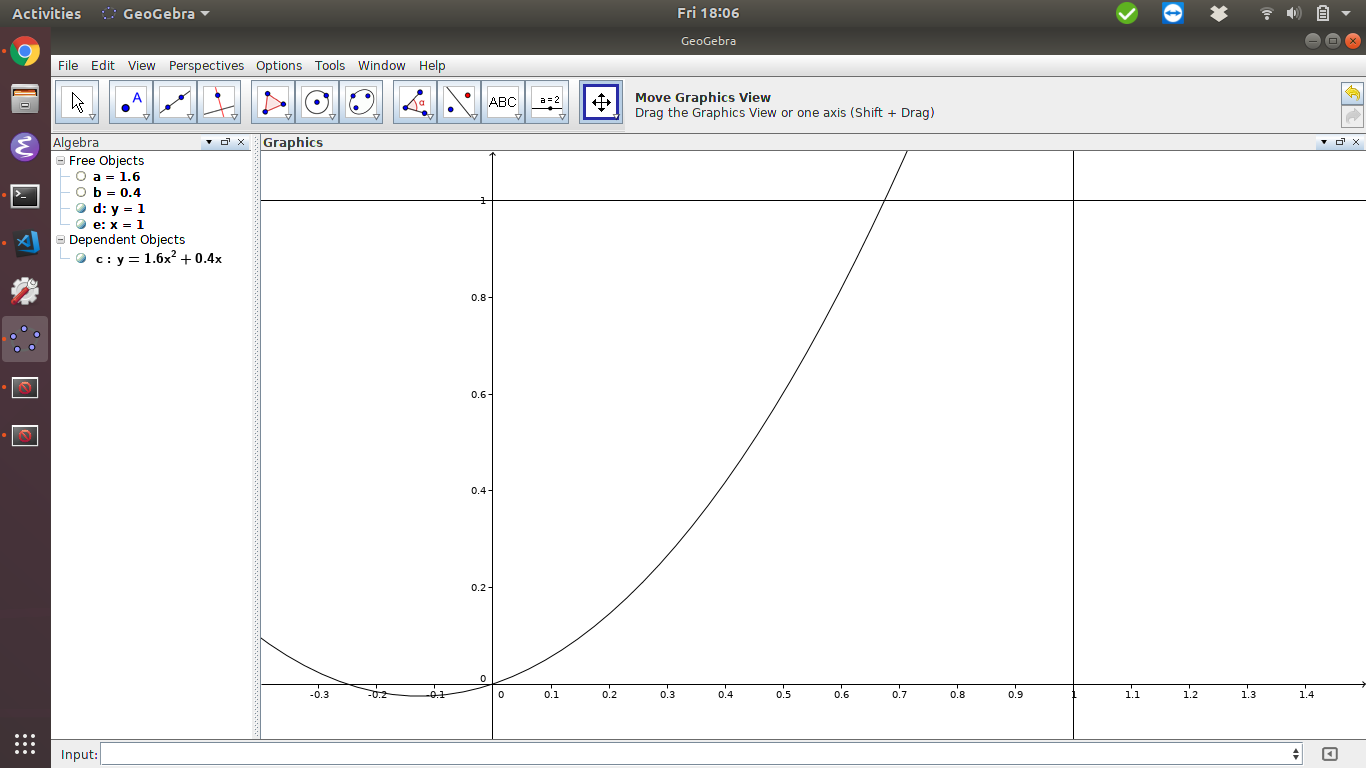
\includegraphics[width=12cm]{modeloCuadratico.png}
%     \caption{Observamos el modelo cuadrático en el software GeoGebra para determinar los parámetros iniciales para nuestra exploración. Con el simulador, los hemos cambiado según nuestras observaciones para que fuera más adecuado al funcionamiento del robot.}
%     \label{fig:modeloCuadratico}
% \end{figure}

\end{document}
